\renewcommand{\arraystretch}{1.5}
\begin{figure}[h]
  \centering
  \begin{tabular}{m{7cm}m{8cm}}
  \toprule
  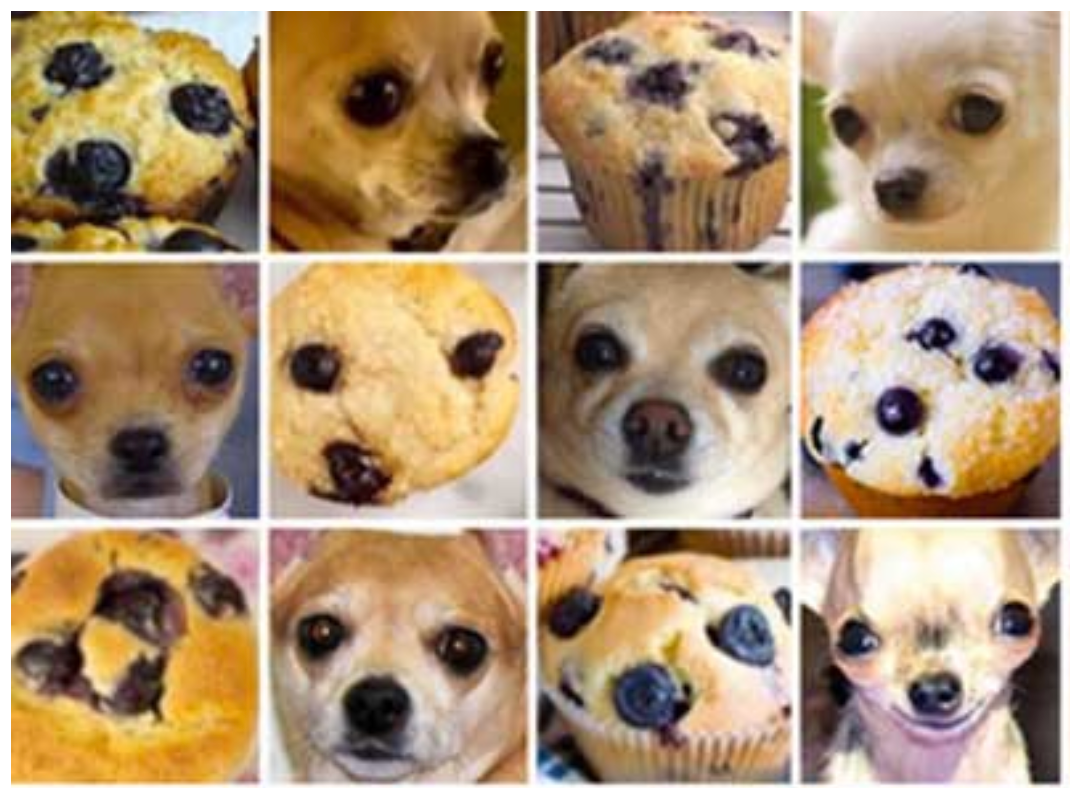
\includegraphics[width=7cm]{figures/example/example4.png} & 
  {\textbf{Instruction:} How many muffin in the image?\par
  \textbf{\mimovlrl{}:} \texttt{<think>...</think>}
To determine the number of muffins in the image, we analyze the 3×4 grid (12 cells total) and count muffins row by row:  

- \textbf{Top row (row 1)}: Columns 1 and 3 are muffins → 2 muffins.  
- \textbf{Middle row (row 2)}: Columns 2 and 4 are muffins → 2 muffins.
- \textbf{Bottom row (row 3)}: Columns 1 and 3 are muffins → 2 muffins. 

Adding these, \( 2 + 2 + 2 = 6 \).  


There are 6 muffins in the image.} \\
\midrule
  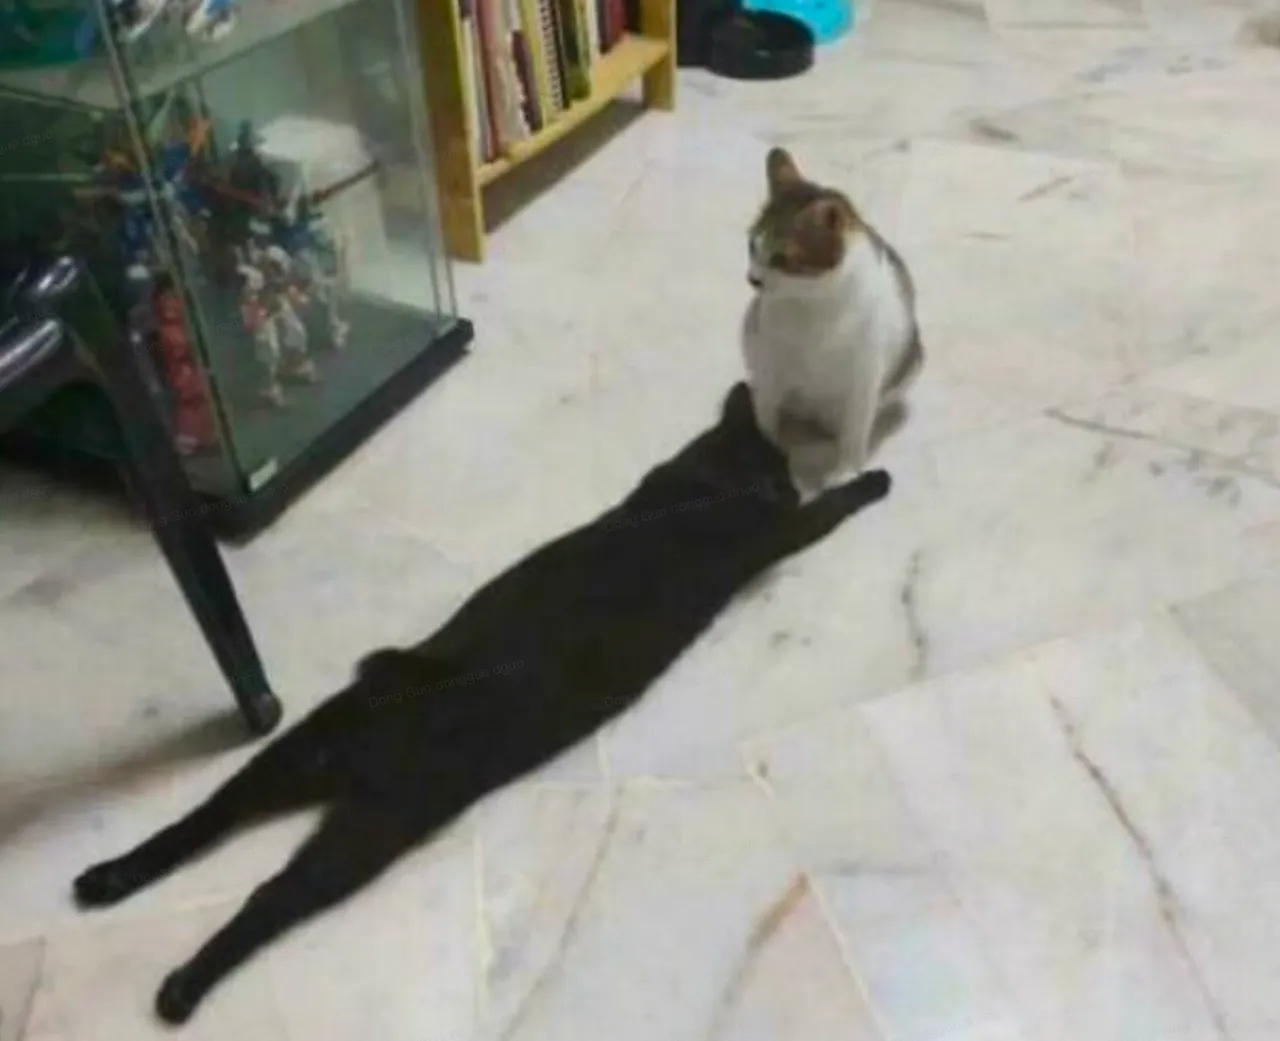
\includegraphics[width=7cm]{figures/example/example5.png} & 
  {\textbf{Instruction:} How many cats in the image?
\par
  \textbf{\mimovlrl{}:} \texttt{<think>...</think>}
To determine the number of cats in the image, we can observe and count:  
- There is a black cat lying on the floor.  
- There is a white and brown cat sitting behind the black cat.  

Thus, the number of cats in the image is 2.  
} \\
\midrule
  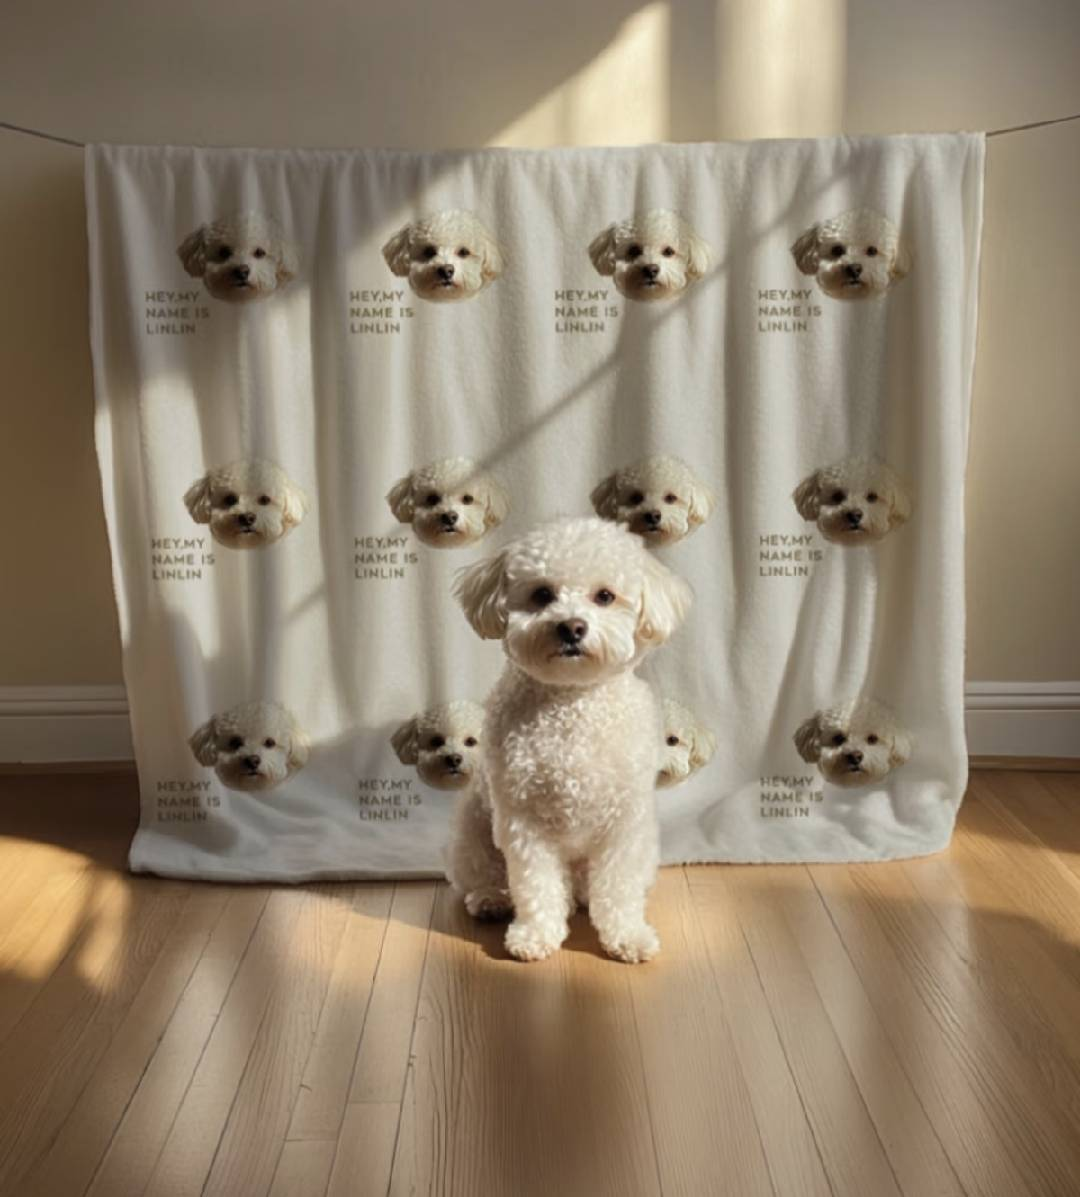
\includegraphics[width=7cm]{figures/example/example6.png} & 
  {\textbf{Instruction:} How many dogs in the image?
\par
  \textbf{\mimovlrl{}:} \texttt{<think>...</think>}
To determine the number of dogs in the image, we analyze both the printed dogs on the blanket and the real dog in the foreground:  
\begin{enumerate}
      \item \textbf{Printed dogs on the blanket}: The blanket features a grid of dog faces. Counting these, we see 3 rows with 4 dogs each, so $ 3 \times 4 = 12 $ printed dogs.  
    \item \textbf{Real dog in the foreground}: There is 1 real dog standing in front of the blanket.    
\end{enumerate}
Adding these together, $ 12 + 1 = 13 $.    

Thus, the total number of dogs in the image is 13.
} \\
  \bottomrule
  \end{tabular}
\caption{Example of \mimovlrl{} solving detailed perception problem.}
\label{fig:case3}
\end{figure}
\renewcommand{\arraystretch}{1}

\clearpage
